\documentclass[sigconf]{acmart}

\usepackage{booktabs} % For formal tables

\DeclareMathOperator*{\argmax}{arg\,max}

\makeatletter
\def\old@comma{,}
\catcode`\,=13
\def,{%
  \ifmmode%
    \old@comma\discretionary{}{}{}%
  \else%
    \old@comma%
  \fi%
}
\makeatother

% Copyright
\setcopyright{none}
%\setcopyright{acmcopyright}
%\setcopyright{acmlicensed}
%\setcopyright{rightsretained}
%\setcopyright{usgov}
%\setcopyright{usgovmixed}
%\setcopyright{cagov}
%\setcopyright{cagovmixed}


% DOI
%\acmDOI{10.475/123_4}

% ISBN
%\acmISBN{123-4567-24-567/08/06}

%Conference
\acmConference[KDD'17]{KDD' 17}{August 13-17}{Halifax, Nova Scotia, Canada} 
\acmYear{2017}
\copyrightyear{2017}

%\acmPrice{15.00}


\begin{document}
\title{Automatic Bayesian Estimation of ARMA Orders}
%\titlenote{Produces the permission block, and
%  copyright information}
%\subtitle{Extended Abstract}
%\subtitlenote{The full version of the author's guide is available as
%  \texttt{acmart.pdf} document}


\author{Skyler Seto}
\affiliation{%
  \institution{Cornell University}
  \streetaddress{Department of Statistical Science}
  \city{Ithaca} 
  \state{New York} 
  \postcode{14853}
}
\email{ss3349@cornell.edu}

\author{Wenyu Zhang}
\affiliation{%
  \institution{Cornell University}
  \streetaddress{Department of Statistical Science}
  \city{Ithaca} 
  \state{New York} 
  \postcode{14853}
}
\email{wz258@cornell.edu}

\author{Andrew Wilson}
\affiliation{%
  \institution{Cornell University}
  \streetaddress{Department of Operations Research and Industrial Engineering}
  \city{Ithaca} 
  \state{New York} 
  \postcode{14853}
}
\email{andrew@cornell.edu}

% The default list of authors is too long for headers}
\renewcommand{\shortauthors}{S. Seto, W. Zhang, A.Wilson}


\begin{abstract}
    An obstacle in employing ARMA models for time series modelling is choosing the correct autoregressive and moving average lag orders $p$ and $q$. This paper proposes ABARMA which uses Bayesian model selection for determining the values of $p$ and $q$ and estimating the model parameters. Evaluating the estimates involves reparametrizing the constrained parameter space and approximating the evidence function using the Laplace method. In simulations, ABARMA performs better or as good as competing methods in all cases. ABARMA exhibits consistent accuracy rates in different noise levels, and becomes increasingly accurate with more observations. In addition, we apply ABARMA on two financial and one seismic activity time series. 
\end{abstract}

%
% The code below should be generated by the tool at
% http://dl.acm.org/ccs.cfm
% Please copy and paste the code instead of the example below. 
%
\iffalse
\begin{CCSXML}
<ccs2012>
 <concept>
  <concept_id>10010520.10010553.10010562</concept_id>
  <concept_desc>Computer systems organization~Embedded systems</concept_desc>
  <concept_significance>500</concept_significance>
 </concept>
 <concept>
  <concept_id>10010520.10010575.10010755</concept_id>
  <concept_desc>Computer systems organization~Redundancy</concept_desc>
  <concept_significance>300</concept_significance>
 </concept>
 <concept>
  <concept_id>10010520.10010553.10010554</concept_id>
  <concept_desc>Computer systems organization~Robotics</concept_desc>
  <concept_significance>100</concept_significance>
 </concept>
 <concept>
  <concept_id>10003033.10003083.10003095</concept_id>
  <concept_desc>Networks~Network reliability</concept_desc>
  <concept_significance>100</concept_significance>
 </concept>
</ccs2012>  
\end{CCSXML}

\ccsdesc[500]{Computer systems organization~Embedded systems}
\ccsdesc[300]{Computer systems organization~Redundancy}
\ccsdesc{Computer systems organization~Robotics}
\ccsdesc[100]{Networks~Network reliability}
\fi
% We no longer use \terms command
%\terms{Theory}

\keywords{ARMA, Bayesian Model Selection}


\maketitle

\section{Introduction}
An autoregressive-moving average model often written ARMA$(p,q)$ describes a stationary discrete-time series $X_t$ using $p$ autoregressive (AR) and $q$ moving average (MA) terms.  The model written recursively satisfies 

\begin{equation*}
\label{arma}
    X_t = \mu + \sum_{j=1}^{p} \phi_{j}X_{t-j} + \sum_{k=1}^{q} \pi_{k}\epsilon_{t-k}+\epsilon_t 
\end{equation*}

where we in general assume $\epsilon_t\sim N(0,\sigma^2)$.  ARMA processes are one of the most general class of models applied to time series  as they model autocorrelated behavior, and can be applied to any stationary time series.

ARMA time series models are a non-standard parametric model as the number of parameters $p + q$ reflected by the order is unknown.  Thus, an obstacle in using ARMA models for forecasting stationary time series is determining the orders $p$ and $q$.  Typically a subjective examination of the partial autocorrelation (pacf) and autocorrelation (acf) functions is used \cite{hyndman2008}.  

Bayesian inference is a natural framework for model selection as it encodes a preference for simpler, more constrained models.  This preference is ideal for ARMA models as typically low order models are sought.  A disadvantage of Bayesian model selection is that the evidence function given by $p(D|M) = \int_{\theta} p(D|\theta)p(\theta|M)\, d\theta$ often needs to be estimated using empirical Bayes approaches or Markov chain Monte Carlo (MCMC), or approximated by Variational Bayes or Laplace approximations.  

In this work, we investigate the feasibility and performance of ABARMA, a fully Bayesian treatment of ARMA model selection.  The ABARMA framework consists of three main components: (1) Bayesian formulation of ARMA model, (2) Reparametrization tricks for intergration over parameter space, (3)Laplace approximation for the evidence function which we delineate in Sections \ref{sec: bayesian}, \ref{sec: reparametrization} and \ref{sec: laplace}. The major contribution of ABARMA over previous Bayesian treatments of ARMA model estimation is that rather than sampling, we provide an analytical approximation to the evidence function for the order selection model using the Laplace approximation. We demonstrate and analyze the accuracy of ABARMA on simulations and real-world data in Sections \ref{sec: simulations} and \ref{sec: real}.


%\end{document}  % This is where a 'short' article might terminate

\section{Related Work}

\subsection{Bayesian Model Selection}

A general strategy for model selection is the Bayesian approach. \cite{minka2000} developed an approach to automatically determine the dimensionality for PCA which shows improved accuracy given sufficient data. Evidence for model $M$ is given as
$$p(D|M) = \int_\theta p(D|\theta)p(\theta|M) d\theta$$
where $D$ denotes the data and $\theta$ denotes the set of parameters corresponding to model $M$. In the PCA model, $M$ is the data dimensionality $k$. The best model is found by maximizing $p(D|k)$ for $k$. The main challenge in this approach is an exact computation or appropriate approximation of the integral.

\subsection{Bayesian ARMA Formulation}
Monahan used the same Bayesian formulation as \cite{minka2000} on ARMA models, where $M$ is uniquely determined by $p$ and $q$, and $\theta=\{\phi_1,\dots,\phi_p,\pi_1,\dots,\pi_q\}$. \cite{monahan1982} $\theta$ is constrained to ensure stationarity and invertibility of the ARMA process, such that the parameter space is analytically intractable for $\min\{p,q\}>4$. Monahan proposed reparametrization of the space to numerically evaluate the integral. Models with $p,q\leq 2$ can be integrated with fixed quadrature rule with extensive bookkeeping of terms, and more complex models are computed by sampling. The paper only assessed the smallest models at $p,q\leq 2$ due to high computational overheads. 

A Bayesian approach with a different objective in the ARMA setting is to derive the posterior distribution of the model parameters $p(\theta|D,M)$. \cite{marriott1993} As in \cite{monahan1982}, the parameter space was reparametrized. A modified Gibbs sampling procedure is used to estimate the posterior distribution.

Another formulation is to consider rewriting an ARMA process as a Gaussian process by rewriting the convariance matrix as a function of the lag orders as in \cite{davis2006} and \cite{rasmussen2005}.  

\subsection{ARMA Model Selection by Information Criteria}

The popular {\tt forecast} {\tt R}  package uses a penalized likelihood (AIC) to assess model fit of a seasonal ARIMA denoted ARIMA$(p,d,q)(P,D,Q)_{m}$ where $m$ is the seasonal frequency, and $d$ and $D$ are the numbers of differencing required such that the resulting series is an ARMA$(p,q)(P,Q)_{m}$ \cite{hyndman2008}. Formally, an ARIMA$(p,d,q)(P,D,Q)_{m}$ is given by
$$\Phi(B^m)\phi(B)(1-B^m)^D(a-B)^dx_t = c+\Theta(B^m)\theta(B)\epsilon_t$$
where $\Phi(z),\phi(z),\Theta(z),\theta(z)$ are polynomials of order $P,p,Q,q$ respectively.
AIC for this SARIMA model is 
$$\text{AIC } = -2log(L)+2(p+q+P+Q+k)$$
where $k=1$ if $c\neq0$ and $k=0$ otherwise.

The model that minimizes the AIC is returned. In view that an exhaustive search for $p,q,P,Q$ is impractical, the {\tt forecast} package uses a step-wise procedure to search the neighborhood of the best model in each step. The AIC explicitly penalizes the number of parameters, such that less complex models are preferred. In practice, especially in cases of complex models, the orders estimated through this method are often less than the true values.

There are many other techniques for ARMA model selection such as {\tt fitARMA} \cite{fitARMA2007}, which uses a fast MLE algorithm to fit an ARMA or ARIMA model,  and {\tt fArma} \cite{fArma2013} which is an alternative package in {\tt R} for fitting and forecasting an ARMA model.  Neither of these packages do any automatic model selection.

\subsection{Other Bayesian Time Series Models}
There are many other bayesian time series models and techniques for forecasting time series data.  We briefly introduce many of these models which have publicly available {\tt R} packages.  

BAYSTAR is a Bayesian modeling procedure for Self-Exciting Threshold AutoRegressive (SETAR) models and Self-Exciting Threshold Vector AutoRegressive (SETVAR) which estimates parameters via MCMC \cite{BAYSTAR2013}.  This model is an extension of a standard AR model and can be viewed as a general piecewise linear approximation.  The general form of a SETAR model is 

$$ y_t = \phi_0^{(j)} + \sum_{i=1}^p \phi_i^{(j)} y_{t-i}n+ \epsilon_t^{(j)}$$

if $y_{t-d} \in R^j$, $j = 1, \dots, M$ where $R^i$ is a partition of the real line, and $d$ is some delay parameter \cite{baystarThesis}. The model does not consider MA terms.

An extension to SETAR and SETVAR is Markov-switching Vector AutoRegressive Models (MSVAR), where properties of the VAR model can vary across regimes according to a hidden Markov chain.  \cite{MSBVAR} utlizes Monte Carlo methods to fit parameters.  An implementation is given in \cite{MSBVARR}.

Another Bayesian modeling procedure is the Bayesian Structural Time Series (BSTS) model.  The general form for a BSTS model is 

$$y_t = Z_t^T\alpha_t + \epsilon_t,  \epsilon_t \sim \mathcal{N}(0,H_t)$$  and $$\alpha_{t+1} = T_t\alpha_t + R_t\eta_t, \eta_t \sim \mathcal{N}(0,Q_t).$$  Typically the matrices $Z_t, T_t$, and $R_t$ contain a mix of known and unknown values \cite{bsts}.  The BSTS model is frequently used when the time series $y_t$ is influenced by exogenous regressors.  An implementation is provided in the {\tt bsts} package in {\tt R} \cite{bstsR}. 

Finally, the {\tt ensembleBMA} package in {\tt R} \cite{BMA} uses Bayeisan model averaging to perform probabilistic forecasting.  {\tt ensembleBMA} fits mixtures of gaussians, mixtures of gammas, and mixtures of gammas with point masses and computes scores for ensemble forecasts.  None of these methods use automatic model selection techniques.



\iffalse
\subsection{Bayesian Optimization for Model Selection}
Bayesian optimization is a strategy for finding the global optimum of a noisy function $f(x): \mathcal{X} \rightarrow R$.  There are two important choices to make when performing Bayesian optimization.  First, one selects a probabalistic model that defines a distribution over functions $f(x)$ to be used to reason about where to search $\mathcal{X}$ for the optimum.  Second, an acquisition function is chosen to quantify the ``potential'' of a new point $x^* \in \mathcal{X}$ \cite{snoek2012}.

Typically, such as in \cite{snoek2012} and \cite{bergstra2011}, Gausian Processes (GP) are used as the prior for $f(x)$ due to their flexibility, and analytic properties.  \cite{snoek2015} developed an approach called Deep Networks for Global Optimization (DNGO) which use Bayesian neural network as a faster alternative to GPs.  DNGO scales linearly in the number of models trained, an improvement over GPs which scales cubically with the number of observations.  One can use Bayesian optimization for hyperparameter selection (and thus model selection) by optimizing a loss function over a bounded parameter space \cite{snoek2015}.
\fi

\begin{table*}[ht]
    \centering
    \begin{tabular}{|c|c|}
    \hline
       $J_{\phi, r}  = \prod_{k=1}^p (1-r_k^2)^{\lfloor \frac{k-1}{2}\rfloor} \prod_{j=1}^{\lfloor \frac{p}{2}\rfloor} (1-r_{2j})$  & $\frac{\partial^2 \log J_{\phi, r}}{\partial \tilde{r}^2_i} = (1-i)[1 - \tanh^2(\tilde{r}_i)]$\\\hline
        $J_{\tilde{r}} =  \prod_{k=1}^p  \left[ 1 - \tanh^2(\tilde{r}_k)\right]$ & $\frac{\partial^2 \log J_{\tilde{r}}}{\partial \tilde{r}_j^2} =  2\tanh^2(\tilde{r}_j) - 2$\\\hline
        $J_{\tilde{\sigma}} = e^{\tilde{\sigma}^2}$ & $\frac{\partial^2 \log J_{\tilde{\sigma}^2}}{\partial (\tilde{\sigma}^2})^2 = 0$\\\hline
    \end{tabular}
    \caption{Second derivatives of $\log$ Jacobians in Equation (4).  $J_{\pi,s}$ and $J_{\tilde{s}}$ are identical. All terms not written are $0$.}
    \label{tab:derivs}
\end{table*}

\section{Bayesian ARMA Model}
\label{sec: bayesian}

In this section, we define the Bayesian formulation for ABARMA.

For simplicity, we assume a mean-zero ARMA process, which is defined as
\begin{equation}
\label{arma2}
    X_t = \sum_{j=1}^{p} \phi_{j}X_{t-j} + \sum_{k=1}^{q} \pi_{k}\epsilon_{t-k}+\epsilon_t 
\end{equation}
where $\epsilon_t$  are i.i.d $N(0,\sigma^2)$ for some constant $\sigma$. We further assume that the unobserved history of the process $\{X_0,X_{-1},\dots,X_{1-p},\epsilon_0,\epsilon_{-1},\epsilon_{1-q}\}$ is $0$. The model $M$ is uniquely determined by $p$ and $q$. Parameters of the model are denoted by $\theta=\{\sigma^2, \phi_1,\dots,\phi_p,\pi_1,\dots,\pi_q\}$.

For a set of $n$ observations $D = \{x_1,x_2,\dots,x_n\}$ from the process $X_t$, the conditional likelihood of the data given the parameters is 

\begin{align*}
    p(D|\theta, M) &= \prod_{i=1}^n p(x_i| x_1,\dots,x_{i-1}, \theta, M)\\
    &= (2\pi \sigma^2)^{-\frac{n}{2}} \exp\left\{-\frac{1}{2\sigma^2}\sum_{t=1}^n (x_t - \mu_t)^2\right\}
\end{align*}

where $\mu_1 = 0$ and $$\mu_t = \sum_{i=1}^p \phi_i x_{t-i} - \sum_{i=1}^q \theta_i(y_{t-i} - \mu_{t-i})$$

as given by \cite{marriott1993}, and the prior density for the parameters is a noninformative prior with $p(\theta | M) \propto \sigma^{-2}$.  

The probability of the data given the model is then computed by integrating over the unknown parameter values in that model to obtain 

\begin{align*}
    \label{evidence}
    p(D|M) &= \int_{\mathcal{U}} p(D|\theta, M) p(\theta | M) \, d\theta\\
    &\propto \int_{\mathcal{U}} \sigma^{-(n+2)} \exp\left\{-\frac{\sum_{t=1}^n (x_t - \mu_t)^2}{2\sigma^2}\right\} \, d\theta \tag{2}
\end{align*}

where the region $\mathcal{U} = \mathbb{R}^+ \times C_p \times C_q$ is over the parameters $\sigma^2$, $\phi$ and $\pi$, and  $$C_p  = \left\{ y_i : \forall w \text{ satisfying } 1 - \sum_{i=1}^p y_i w^i = 0, |w| > 1 \right\}$$ is the region of $\phi$'s and $C_q$ is the region of $\theta$'s such that $X_t$ is a stationary and identifiable process \cite{monahan1982}. 

Computing the evidence over the restricted regions $C_p$ and  $C_q$ is difficult since for $p$ or $q > 4$, $C_p$ cannot be written and integrated over nicely \cite{marriott1993}.     To evaluate the integral a reparametrization of the $\phi$'s and $\theta$'s which maps the region $C_p \times C_q \rightarrow \mathbb{R}^{p+q}$ is proposed. We also include a reparametrization of $\sigma^2$ which maps $\mathbb{R}^+ \rightarrow \mathbb{R}$. We then approximate the new integral  over $\mathbb{R}^{p+q+1}$ via the Laplace approximation.  The optimal model is chosen as
$$M_{opt} = \argmax_{M} p(D|M).$$


\section{Reparametrization Tricks}
\label{sec: reparametrization}

To integrate over the restricted region $C_p \times C_q$, two successive transformations are proposed as in \cite{marriott1993}.  We adopt the first transformation, and make a modification on the second. The first is the transformation between $\phi \in C_p$ and $r = (r_1, r_2, \dots, r_p)$ with $|r_i|<1$ for all $i$ proposed by \cite{marriott1993} and written as

\begin{align*}
    \phi_k^{(k)} &= r_k\\
    \phi_i^{(k)} &= \phi_i^{(k-1)} - r_k \phi_{k-i}^{(k-1)} \tag{for $i=1, \dots, k-1$}
\end{align*}

where $\phi_i^{(p)}$ is the $i$th coefficient from the ARMA$(p,q)$ process.  Note that an identical parametrization can be done for $(\pi_1, \dots, \pi_q)  \in C^q$ to $s = (s_1, s_2, \dots, s_q)$ with $|s_i| < 1$ for all $i$.

The second reparametrizaion maps each $r_i$ to $\tilde{r}_i \in \mathbb{R}$.  Here any function mapping from $(-1, 1) \rightarrow \mathbb{R}$ will work.  We take $\tilde{r}_i = \tanh^{-1}\left(r_i\right)$ for two reasons:

\begin{enumerate}
    \item The inverse transformation $r_i = \tanh(\tilde{r}_i)$ can be easily differentiated.  This will be useful for analytically deriving the Jacobian and Hessian in the next section.
    
    \item Due to the stationarity and invertibility constraints, we expect the $\tilde{r}_i$'s to be small. The gradient of $\tanh$ is close to zero only when $\tilde{r}_i$ is large in magnitude. Hence we tend to avoid getting stuck in areas of zero gradient when optimizing the objective function containing $\tanh$.
\end{enumerate}

Again, we can do an identical transformation from $s_i$ to $\tilde{s}_i \in \mathbb{R}$.

Lastly we transform $\sigma^2\in \mathbb{R}^+$ to $\tilde{\sigma}^2\in \mathbb{R}$ by
$\tilde{\sigma}^2 = \log(\sigma^2)$
such that the parameter space is the entire $\mathbb{R}^{p+q+1}$. This makes the Laplace approximation more reasonable, since we would like to use a multivariate Gaussian to approximate our objective function and multivariate Gaussians have parameter support over the entire Euclidean space.

The transformed integral for the evidence function can now be written as 

\begin{align*}
    p(D|M) &=  \int_{\mathcal{U}} p(D|\theta, M) p(\theta | M) \, d\theta\\
    &= \int_{\tilde{\mathcal{U}}} p(D|\theta^*, M) p(\theta^* | M) J_{\theta^*} \, d\theta^* \tag{3}
\end{align*}

where $\tilde{\mathcal{U}} = \mathbb{R}^{p+q+1}$, $\theta^* = \{\tilde{\sigma}^2, \tilde{r}_1, \dots, \tilde{r}_p, \tilde{s}_1, \dots, \tilde{s}_q \}$ and $J_{\theta^*} = J_{\phi, r} J_{\pi, s} J_{\tilde{r}} J_{\tilde{s}} J_{\tilde{\sigma}}$ is the product of the Jacobians for each transformation.  The Jacobians are written in Table \ref{tab:derivs}.

An explicit form for $p(D|\theta^*, M)p(\theta^*|M)$ is given by 

\begin{align*}\log p(D,\theta^*|M) \propto -\frac{n+2}{2}\tilde{\sigma}^2 -\frac{1}{2}e^{-\tilde{\sigma}^2}\sum_{t=1}^n (x_t - \tilde{\mu}_t)^2 \end{align*}

\begin{align*}\tilde{\mu}_t = \sum_{i=1}^p \phi_i(\tilde{r}) x_{t-i} - \sum_{i=1}^q \pi_i(\tilde{s})(x_{t-i}-\tilde{\mu}_{t-i}) \end{align*}

where the above expressions are parametrized by $\phi$'s and $\pi$'s as functions of $\tilde{r}$'s and $\tilde{s}$'s respectively, and $\sigma^2$ as $\tilde{\sigma}^2$.   Computationally the functions $\phi(\tilde{r})$ and $\pi(\tilde{s})$ can be computed recursively given $\tilde{r}_1, \dots, \tilde{r}_p, \tilde{s}_1, \dots, \tilde{s}_q$.

\iffalse
We obtain $J_{\phi, r}$  from Equation (7) of \cite{marriott1993} as

$$J_{\phi, r}  = \prod_{k=1}^p (1-r_k^2)^{\lfloor \frac{k-1}{2}\rfloor} \prod_{j=1}^{\lfloor \frac{p}{2}\rfloor} (1-r_{2j})$$

  We derive the Jacobians corresponding to the second transformation as

$$J_{\tilde{r}} =  \prod_{k=1}^p  \left[ 1 - \tanh^2(\tilde{r}_k)\right] .$$

Both $J_{\pi, s}$ and $J_{\tilde{s}}$ can be written identically.  Lastly, $J_{\tilde{\sigma}} = e^{\tilde{\sigma}^2}$.
\fi

\begin{table*}[t]
    \centering
    \begin{tabular}{|c|c|}
    \hline
       $\frac{\partial^2 \log p(D,\theta^*|M)}{\partial \tilde{r}_j\tilde{r}_i}$ & $e^{-\tilde{\sigma}^2}\sum_{t=1}^n \left( (x_t-\tilde{\mu}_t)\frac{\partial^2 \tilde{\mu}_t}{\partial \tilde{r}_j\partial \tilde{r}_i} - \frac{\partial \tilde{\mu}_t}{\partial \tilde{r}_j} \frac{\partial \tilde{\mu}_t}{\partial \tilde{r}_i} \right)$\\\hline
       $\frac{\partial^2 \log p(D,\theta^*|M)}{\partial \tilde{s}_j\tilde{r}_i}$ & $e^{-\tilde{\sigma}^2}\sum_{t=1}^n \left( (x_t-\tilde{\mu}_t)\frac{\partial^2 \tilde{\mu}_t}{\partial \tilde{s}_j\partial \tilde{r}_i} - \frac{\partial \tilde{\mu}_t}{\partial \tilde{s}_j} \frac{\partial \tilde{\mu}_t}{\partial \tilde{r}_i} \right)$\\\hline
       $\frac{\partial^2 \log p(D,\theta^*|M)}{\partial \sigma^2 \partial \tilde{r}_i}$ & $-e^{-\tilde{\sigma}^2}\sum_{t=1}^n (x_t-\tilde{\mu}_t)\frac{\partial \tilde{\mu}_t}{\partial \tilde{r}_i}$\\\hline
       $\frac{\partial^2 \log p(D,\theta^*|M)}{\partial (\sigma^2)^2}$ & $-\frac{1}{2}e^{-\tilde{\sigma}^2} \sum_{t=1}^n (x_t-\tilde{\mu}_t)^2$\\\hline
        $\frac{\partial^2 \tilde{\mu}_t}{\partial \tilde{r}_j \partial \tilde{r}_i}$ & $\sum_{l=1}^p \frac{\partial^2 \phi_l(\tilde{r})}{\partial \tilde{r}_j \partial \tilde{r}_i} x_{t-l} + \sum_{l=1}^q \pi_l(\tilde{s}) \frac{\partial^2 \tilde{\mu}_{t-l}}{\partial \tilde{r}_j \partial \tilde{r}_i}$\\\hline
    $\frac{\partial^2 \tilde{\mu}_t}{\partial \tilde{s}_j \tilde{s}_i}$ & $\sum_{l=1}^q \left( \pi_l(\tilde{s})\frac{\partial^2 \tilde{\mu}_{t-l}}{\partial \tilde{s}_j \partial \tilde{s}_i} + \frac{\partial \tilde{\mu}_{t-l}}{\partial \tilde{s}_i}\frac{\partial \pi_l(\tilde{s})}{\partial \tilde{s}_j} + (\tilde{\mu}_{t-l}-x_{t-l})\frac{\partial^2 \pi_l(\tilde{s})}{\partial \tilde{s}_j \partial \tilde{s}_i} + \frac{\partial \pi_l(\tilde{s})}{\partial \tilde{s}_i} \frac{\partial \tilde{\mu}_{t-l}}{\partial \tilde{s}_j} \right)$\\\hline
    $\frac{\partial^2 \tilde{\mu}_t}{\partial \tilde{s}_j \partial \tilde{r}_i}$ & $\sum_{l=1}^q\left( \pi_l(\tilde{s})\frac{\partial \tilde{\mu}_{t-l}}{\partial \tilde{s}_j \partial \tilde{r}_i} + \frac{\partial \pi_l(\tilde{s})}{\partial \tilde{s}_j}\frac{\partial \tilde{\mu}_{t-l}}{\partial \tilde{r}_i} \right)$\\\hline
    \end{tabular}
    \caption{Second derivatives of $\log\left(p(D, \theta^* |  M)\right)$.}
    \label{tab:pdmderivs}
\end{table*}

\section{Laplace Approximation} 
\label{sec: laplace}

The Laplace method is an approach for approximating an integral based on its derivatives.  Suppose we would like to approximate $\int f(x)\, dx$ where $f(x)$ has a mode at $\hat{x} = \argmax_x f(x)$.  We write the Taylor expansion for $\log(f(x))$ about $\hat{x}$:

$$\log(f(x)) \approx \log f(\hat{x}) - \frac{1}{2} (x - \hat{x})^TH(x - \hat{x})$$

where $H$ is the Hessian matrix with $$H_{i,j} = \left[\frac{\partial^2 \log(f(x))}{\partial x_i \partial x_j}\right]_{x = \hat{x}}.$$

Then, we have that 

\begin{align*}
    \int f(x) \, dx &\approx f(\hat{x}) \int \exp\left\{  - \frac{1}{2} (x - \hat{x})^TH(x - \hat{x})\right\}\, dx\\
    &=  f(\hat{x}) (2\pi)^{\text{rows}(H)/2} |-H|^{-\frac{1}{2}}
\end{align*}

as given by \cite{minka2000} Equation (37).  
It suffices to compute the second derivative over all $\theta^*_i$ and $\theta^*_j$ of

\begin{align*}
    \log f(\theta^*) &= \log\left(p(D|\theta^*, M)p(\theta^* | M)\right)  + \log J_{\theta^*} + C\\
    &= \log\left(p(D, \theta^* |  M)\right) +  \log J_{\phi, r} \tag{4}\\
    &+ \log  J_{\pi, s} + \log J_{\tilde{r}}  + \log J_{\tilde{s}} + \log J_{\tilde{\sigma}} + C
\end{align*}

yielding the evidence function approximation

\begin{align*}
    p(D|M) \approx f(\hat{\theta^*}) (2\pi)^{\text{rows}(H)/2} |-H|^{-\frac{1}{2}} \tag{5}
\end{align*}

where $H$ is the hessian of (4) evaluated at $\hat{\theta^*}$.

The second derivative of the $\log$ of the Jacobians are given in Table \ref{tab:derivs}.  The second derivatives of $\log\left(p(D, \theta^* |  M)\right)$ with respect to $\tilde{r}$, $\tilde{s}$, and $\tilde{\sigma}^2$ are summarized in Table \ref{tab:pdmderivs}.  All other second derivatives are zero.
 
 
 
\iffalse
 The second derivative of $\log J_{\tilde{\sigma}}$ with respect to any of the variables in $\theta^*$ is $0$.  Equations (2B) and (3B) from Appendix B give the expressions for the second derivatives of the other Jacobian terms in (4).  Appendix A derives recursive equations for the second derivative and shows an example of these derivations for first derivative when $p, q=3$.  The second derivative for this particular example can easily be computed.
 \fi
 Figure \ref{fig:laplace} shows $f(\theta^*)$ for an AR$(1)$ process. Since the graph is roughly normal, the Laplace approximation is a reasonable approximation.  We expect this is the case for higher order processes as well.

\begin{figure}
    \centering
    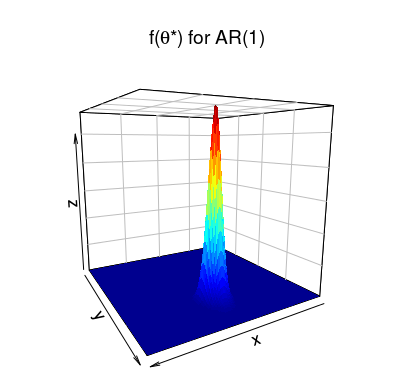
\includegraphics[width=2in]{ar1Laplace_v2.png}
    \caption{Laplace Approximation for AR$(1)$ process}
    \label{fig:laplace}
\end{figure}

Finally, to find the optimal $p$ and $q$ a simple grid search procedure is employed on the expression on the right hand side of (5).  Extensions to this optimization procedure are discussed in Section \ref{sec: conclusion}.

\iffalse
\section{Alternative Approximations}
Rather than approximating the expression in (3) we consider approximating the region $C_p \times C_q$ by a region we can more easily integrate over or reparametrize.  The approximated region for $C_3$ is briefly described as follows.  
\cite{monahan1982} describes the region $C_2$ as the interior of the triangle with vertices $(\pm 2, -1)$ and $(1,0)$. Thus, we know that $C_3$ must contain all points of the form $(\phi_1, \phi_2, 0)$ where $(\phi_1, \phi_2)$ is in the interior of the triangle.  Further, by the Vieta formulas we know an exact value for the product of the roots of the polynomial and thus $\phi_3 \in (-1, 1)$.  Using this, we can approximate $C_3$ as a triangular pyramid based on the assumption the region is enclosed by linear planes.  
\fi

\section{Parameter Estimation}
\label{sec: params}
After determining the model $M$, we can obtain the posterior distribution of the parameters $\theta$ by
\begin{align*}
    p(\theta|M,D) 
    &= \frac{P(D|\theta,M)P(\theta|M)}{P(D|M)} \\
    &= \frac{P(D|\theta^*,M)P(\theta^*|M)J_{\theta^*}}{P(D|M)} 
\end{align*}
    
One point estimate of $\theta$ is the argmax of the posterior distribution. $\hat{\theta}^* = \argmax_{\theta^*} P(D|\theta^*,M)P(\theta^*|M)J_{\theta^*}$ is found when calculating the mode of equation (4). Therefore, we obtain an estimate of the model parameters as a byproduct of the Laplace method used to approximate the ARMA lag orders.

Other estimates such as posterior means require more computational work.

\section{Simulations}
\label{sec: simulations}

We implement the ABARMA procedure in {\tt R} using the {\tt optim} function in base {\tt R} to compute $\hat{\theta^*} = \argmax f(\theta^*)$ and $H$ at $\hat{\theta^*}$.

To evaluate the performance of ABARMA for ARMA model selection, data is sampled from a known ARMA$(p,q)$ model using the {\tt arima.sim} function in {\tt R} and we fit the series by the ABARMA procedure.  We evaluate the ABARMA algorithm by measuring the runtime, model forecast accuracy (measured by RMSE), and the closeness of the determined lag orders from the true model lag orders.  To compute the forecast accuracy, we used the {\tt arima} function in base {\tt R} to approximate the parameters based on the determined model, and used the {\tt forecast} function from the {\tt forecast} package to predict future observations.

The three estimators AIC, BIC, and AICc used by the {\tt auto.arima} function in {\tt R}, the maximum likelihood estimator, and one-fold cross validation are used for comparison.  In the latter method, the model is trained by withholding the last $20\%$ of the series and minimizing the Root-Mean-Square Error (RMSE) on the withheld set.  

We tested the performance of ABARMA under different time series length and noise levels, as well as the robustness of the method to different initializations for finding the mode $\hat{\theta^*}$. Additionally, we tested the ability of ABARMA in estimating model parameters from the Laplace approximation procedure as described in Section \ref{sec: params}.

Except in Section \ref{sec: length} where the series length is varied, all simulated time series in this section have length $n=100$, and forecast length is $20$. This choice is made because the competing methods in the {\tt auto.arima} function approximate the maximum likelihood when the number of observations exceeds $100$. For length 100 series, ABARMA takes approximately 6 minutes on a standard desktop computer to perform grid search over all $p$ and $q$. All competing methods take on the order of 25 seconds.  ABARMA is relatively slower since finding the optimal $p$ and $q$ requires numerically computing  $\hat{\theta^*} = \argmax f(\theta^*)$ which can have slow convergence in some cases.  We do not compare our model to that proposed in \cite{monahan1982} as it is based on numerical integration which is very slow.  For particular values of $p$ and $q$ the numerical integration can take several minutes alone.

To improve the efficiency of the algorithm a procedure identical to the step-wise procedure in \cite{hyndman2008} is implemented.  This brings the runtime to on average 4 seconds for an ARMA$(2,1)$ model, 14 seconds for an ARMA$(5,3)$ model, and 25 seconds for an ARMA$(8,6)$ model.  We elaborate more on the accuracy of the step-wise procedure in Section \ref{sec:speedups} but note that the accuracy stays roughly the same, except in the ARMA$(8,6)$ models where we see a small decrease in accuracy.
 

\subsection{Model Complexity}
\label{sec: complexity}

We simulate a mean zero series from each of model orders: $p, q = (2,1)$ and $(5,3),$ and $(8,6)$ which we label low, medium, and high order models respectively. Examples of these series are shown in Figure \ref{sample}.

\begin{figure}
    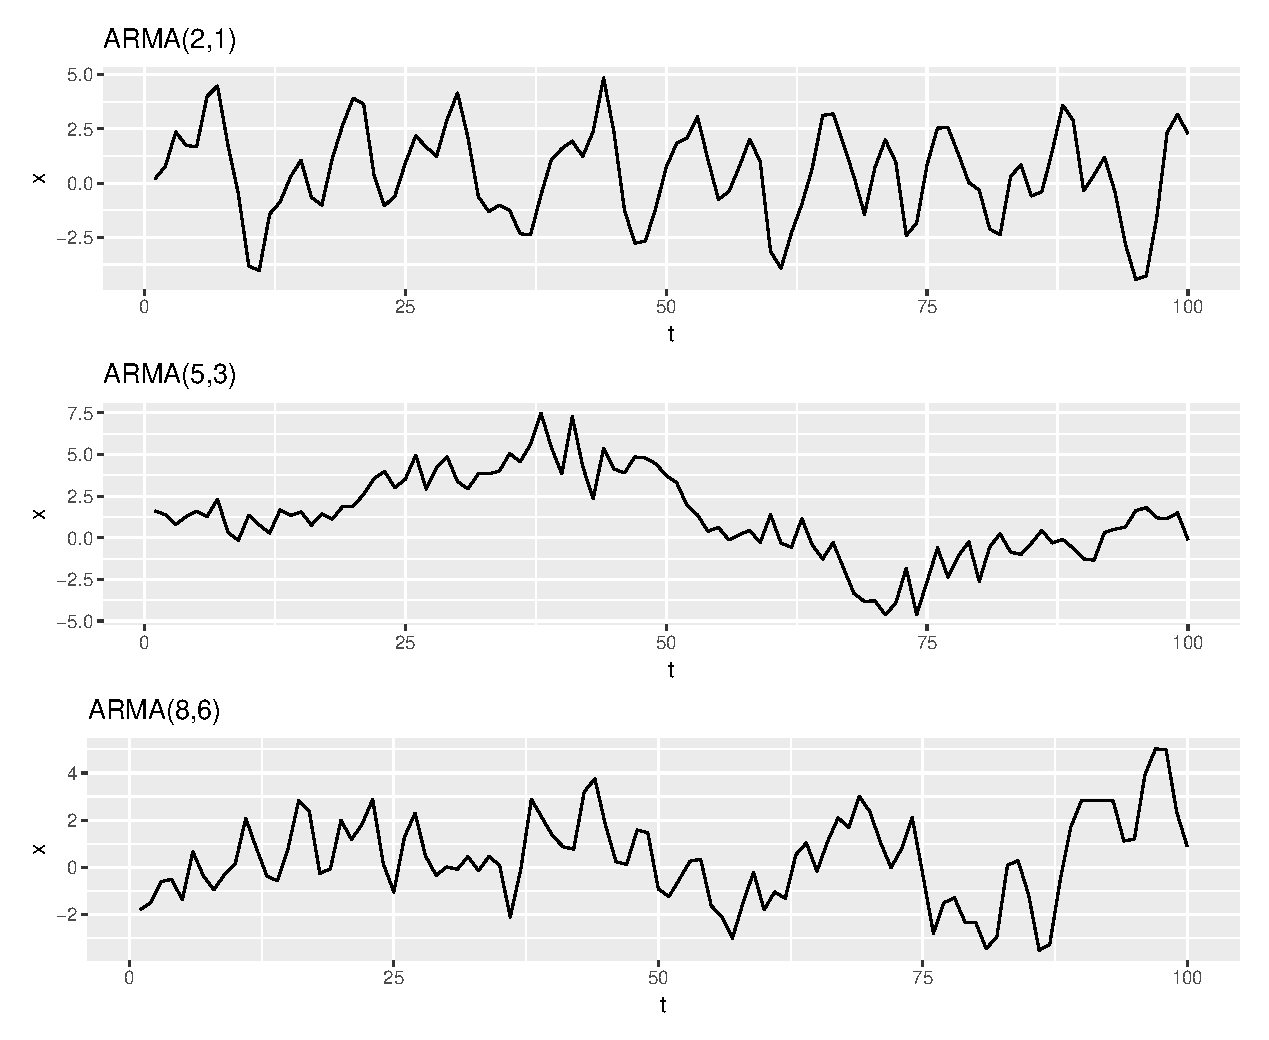
\includegraphics[width=3in]{armaLMH.eps}
    \caption{Top: ARMA$(2,1)$, Middle: ARMA$(5,3)$, Bottom: ARMA$(8,6)$}
    \label{sample}
\end{figure}

For each choice of $p$ and $q$, Figures \ref{heatmap21_v2}, \ref{heatmap53_v2}, and \ref{heatmap86_v2} plot the scores given by the various estimators. The higher the score, the darker the blue color. A grey square indicates a $NaN$ score, due to non-convergence of the {\tt optim} function. From the figures, we observe that ABARMA places significantly higher scores at and near the true model orders, while all other methods either place an almost uniform distribution over most $p$ and $q$ or are far off from the true model orders.

\begin{figure}
    \centering
    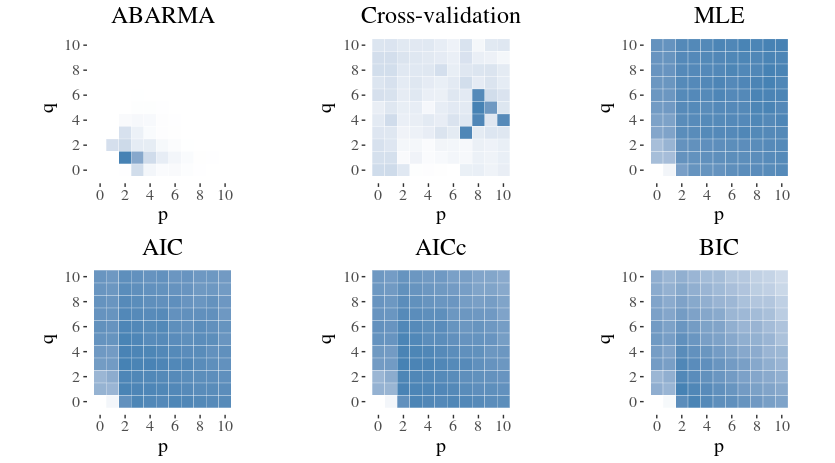
\includegraphics[width=3.3in]{heatmap21_v2.png}
    \caption{Scores for ARMA(2,1)}
    \label{heatmap21_v2}
\end{figure}

\begin{figure}
    \centering
    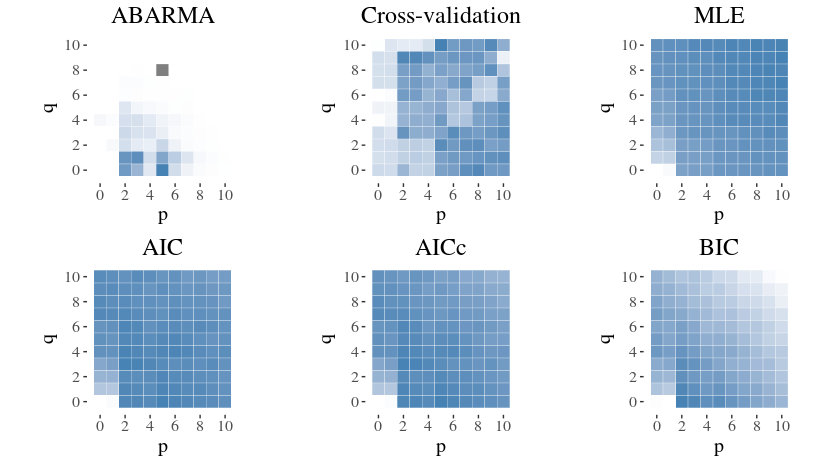
\includegraphics[width=3.3in]{heatmap53_v2.png}
    \caption{Scores for ARMA(5,3)}
    \label{heatmap53_v2}
\end{figure}

\begin{figure}
    \centering
    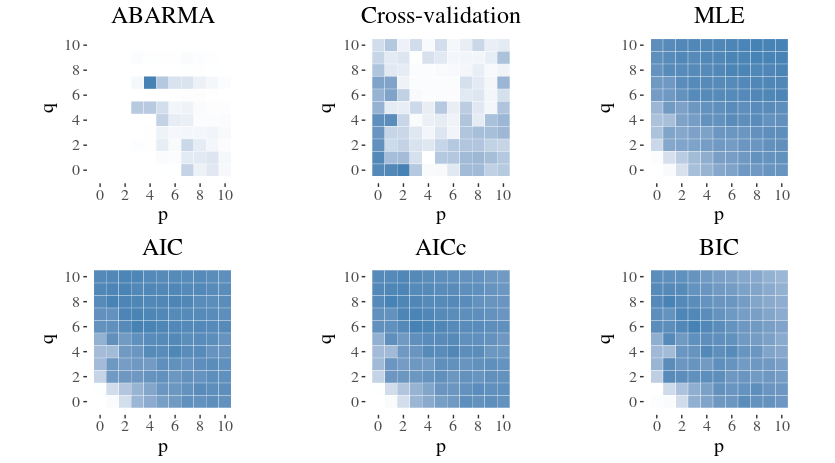
\includegraphics[width=3.3in]{heatmap86_v3.png}
    \caption{Scores for ARMA(8,6)}
    \label{heatmap86_v2}
\end{figure}

We replicate the above simulations 25 times, with results in Figures \ref{lagplot21} to \ref{foreplot86}. In each of the three different orders, the ABARMA procedure correctly identifies the correct orders more often than all other methods. ABARMA is also better or at least as good as the other methods in precisely and accurately forecasting future observations.

\begin{figure}
    \centering
    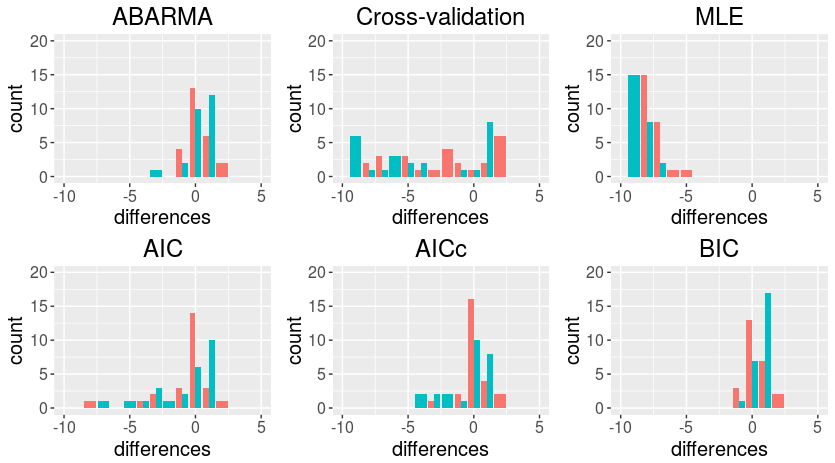
\includegraphics[width=3.3in]{truelag-approxlag21.png}
    \caption{True Lag Orders - Approximated Lag Orders for ARMA(2,1). Red for p, blue for q.}
    \label{lagplot21}
\end{figure}

\begin{figure}
    \centering
    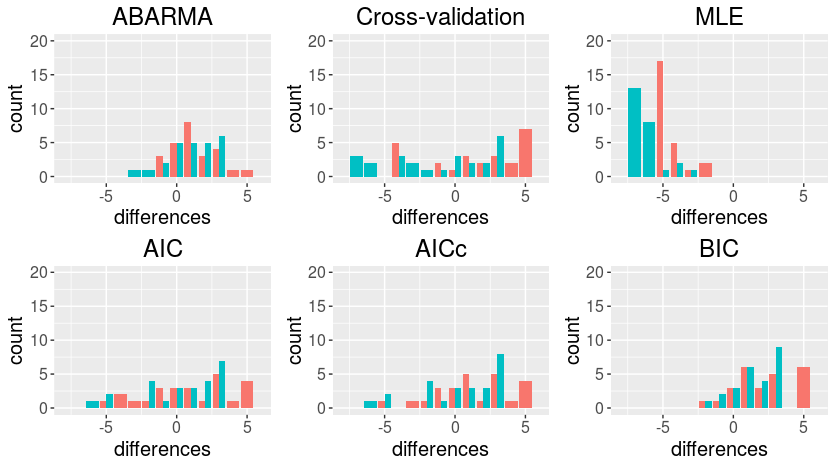
\includegraphics[width=3.3in]{truelag-approxlag53.png}
    \caption{True Lag Orders - Approximated Lag Orders for ARMA(5,3). Red for p, blue for q.}
    \label{lagplot53}
\end{figure}

\begin{figure}
    \centering
    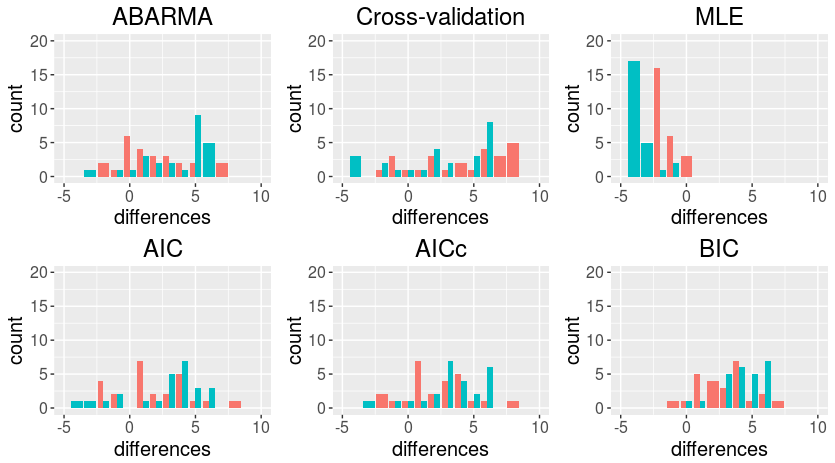
\includegraphics[width=3.3in]{truelag-approxlag86.png}
    \caption{True Lag Orders - Approximated Lag Orders for ARMA(8,6). Red for p, blue for q.}
    \label{lagplot86}
\end{figure}

\begin{figure}
    \centering
    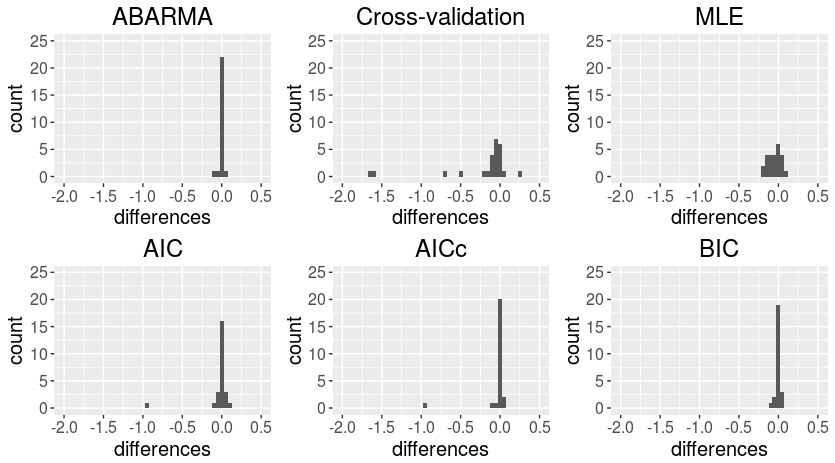
\includegraphics[width=3.3in]{truefore-modelfore21.png}
    \caption{Forecast Errors of True Model - Forecast Errors of Approximated Models for ARMA(2,1).}
    \label{foreplot21}
\end{figure}

\begin{figure}
    \centering
    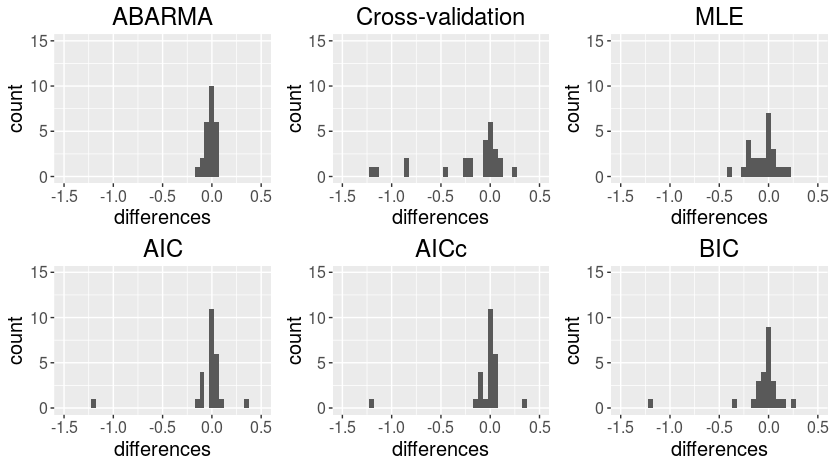
\includegraphics[width=3.3in]{truefore-modelfore53.png}
    \caption{Forecast Errors of True Model - Forecast Errors of Approximated Models for ARMA(5,3).}
    \label{foreplot53}
\end{figure}

\begin{figure}
    \centering
    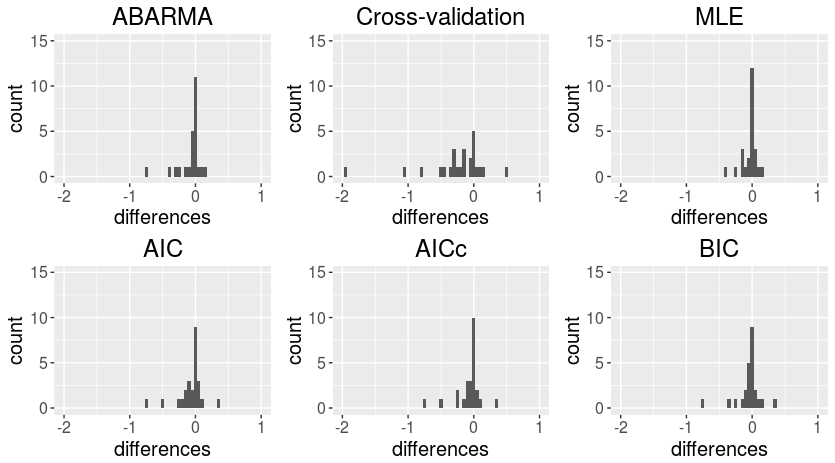
\includegraphics[width=3.3in]{truefore-modelfore86.png}
    \caption{Forecast Errors of True Model - Forecast Errors of Approximated Models for ARMA(8,6).}
    \label{foreplot86}
\end{figure}


\subsection{Length of Series}
\label{sec: length}

We conduct the experiment on 10 ARMA(2,1) series of length 100 and 200 respectively. Figure \ref{length21} shows the accuracy of each method in simultaneously estimating both $p$ and $q$ correctly. ABARMA's accuracy is higher than those of all other methods, and it increases with series length, as is expected from the Bayesian formulation of the problem.  We also note that the runtime scales linear with the length of the series indicating this is a potential shortcoming of the model.

\begin{figure}
    \centering
    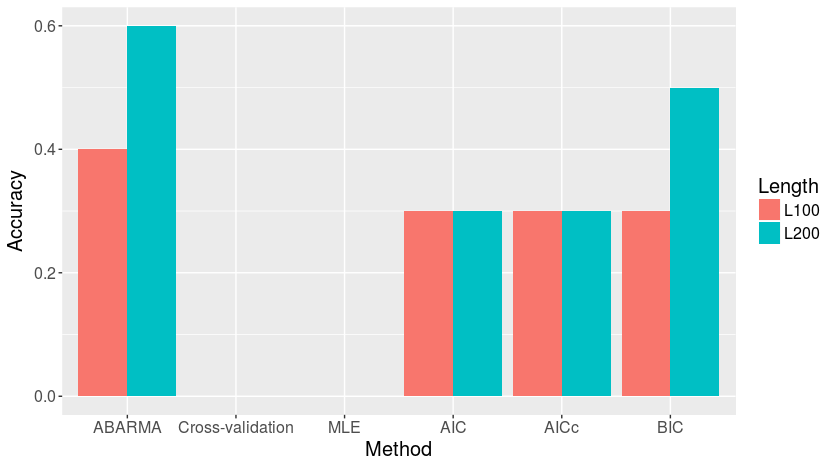
\includegraphics[width=3in]{length21.png}
    \caption{Lag Order Approximation Accuracy against Length of Time Series.}
    \label{length21}
\end{figure}


\subsection{Noise Level}

We simulate 10 ARMA(2,1) series with three different noise levels respectively. That is, for the error term $\epsilon_t \sim \mathcal{N}(0,\sigma^2)$, we set $\sigma^2 = 1,5,$ and $10$. The percentage accuracies plotted in Figure \ref{noise21} show that ABARMA is consistent in its estimation accuracy across the three noise levels, and that ABARMA is more accurate or at least as accurate as the other methods in all three scenarios.  There is no change in runtime accompanying a change in noise.

\begin{figure}
    \centering
    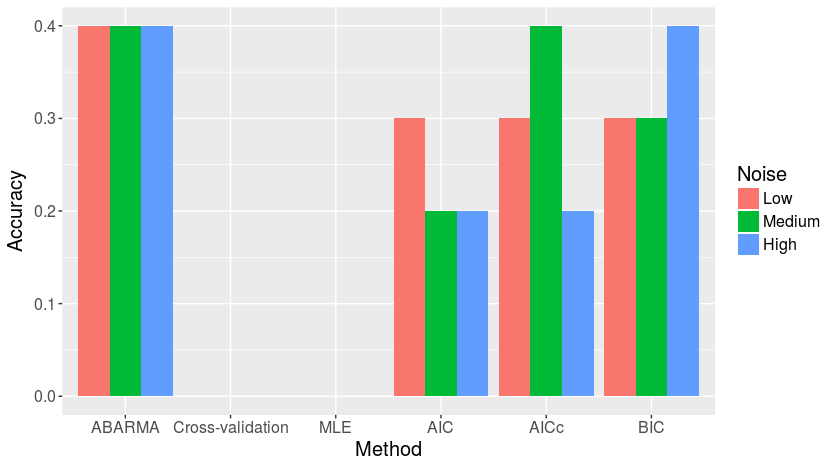
\includegraphics[width=3in]{noise21.png}
    \caption{Lag Order Approximation Accuracy against Noise Level.}
    \label{noise21}
\end{figure}

\subsection{Robustness to Initializations}
We additionally experiment with different intializations for the ABARMA procedure.  We test five different series with 10 different initializations for an ARMA$(2,1)$ process.  Figure \ref{init21} shows the results of choosing initializations uniformly for finding $\hat{\theta^*}$.  There is little to no difference between different initializations, and the default initialization (all zeroes) for the coefficients is according to the majority selection. 
\begin{figure}
    \centering
    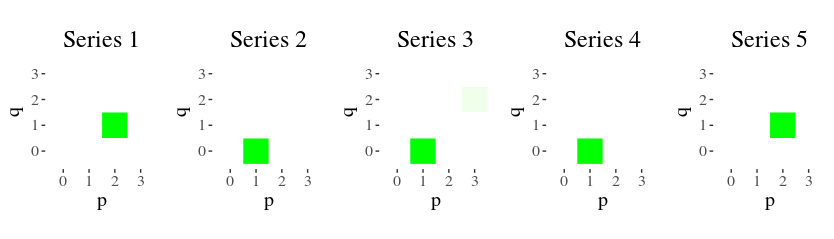
\includegraphics[width=3.25in]{init21.png}
    \caption{Model estimations with random initializations. Initializing at 0 gives (2,1) for Series 1, (1,0) for Series 2, 3 and 4, and (2,1) for Series 5. }
    \label{init21}
\end{figure}

\subsection{Model Parameter Approximation}

For 10 ARMA(1,1) series where ABARMA accurately approximates the model orders, we further estimate the model parameters $\phi,\pi$ and $\sigma^2$ by the method described in Section \ref{sec: params}. The first two plots in Figure \ref{paramplot} show that the estimated lag coefficients are close to the true ones. The third plot shows that the estimated $\sigma^2$ is close to the true noise variance 1. 

\begin{figure}
    \centering
    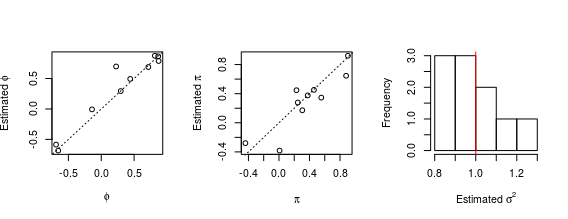
\includegraphics[width=3.25in]{paramplot.png}
    \caption{Estimated $\phi,\pi$ Coefficients against True $\phi,\pi$ Coefficients for ARMA(1,1). Histogram of Estimated $\sigma^2$, true $\sigma^2=1$ indicated by red line.}
    \label{paramplot}
\end{figure}

\subsection{Potential Computational Speedups}
\label{sec:speedups}
We implement Stepwise-ABARMA on the same simulated examples from Section \ref{sec: complexity}.  Figure \ref{stepwise} shows the lag order approximation results where the stepwise procedure is initiated and performed according to \cite{hyndman2008}. We notice that Stepwise-ABARMA has similar performance to the non-stepwise version in the low and medium order cases, since the initialization is at low order models.  We consider changing the initialization to start at the maximum $p(D|M)$ where $M = (p,q) \in \{(1,1), (5,5), (9,9)\}$.   Figure \ref{stepwise2} shows that as expected there is improvement when the series is higher order, but there is a slight decrease in accuracy when the series is low or medium order.  As the model may start at an incorrect initialization, the overall average runtime is also slightly higher at 30 seconds for low order models, 45 seconds for medium order models, and 78 seconds for high order models. 

\begin{figure}
    \centering
    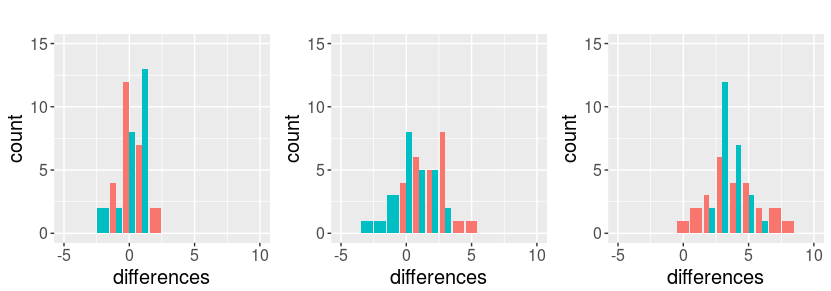
\includegraphics[width=3.25in]{stepwise.png}
    \caption{True Lag Orders - Approximated Lag Orders by Stepwise-ABARMA for ARMA(2,1) (left), ARMA(5,3) (center), and ARMA(8,6) (right). Red for p, blue for q.}
    \label{stepwise}
\end{figure}


\begin{figure}
    \centering
    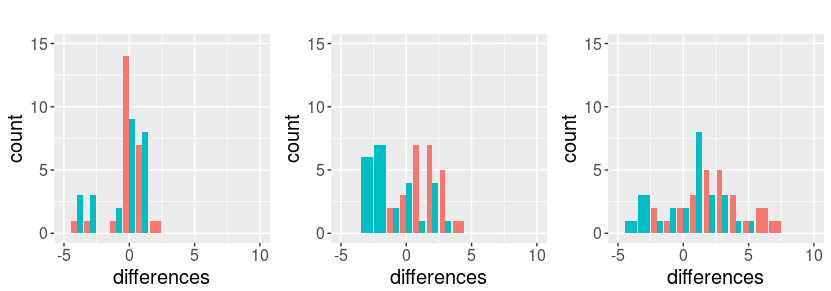
\includegraphics[width=3.25in]{stepwise2.png}
    \caption{True Lag Orders - Approximated Lag Orders by Stepwise-ABARMA for ARMA(2,1) (left), ARMA(5,3) (center), and ARMA(8,6) (right) using $\max\{(1,1), (5,5), (9,9)\}$ initialization. Red for p, blue for q.}
    \label{stepwise2}
\end{figure}

Using the step-wise procedure with ``IC'' based methods also greatly reduces the runtime of the method to udner one second, however for medium and high order models accuracy drops.  The methods tend to favor lower order models with aic selecting a model with $p\geq 4$ five times out of twenty-five, and bic selecting a model three times.  These models tend to favor more parsimonius models and it is expected these models will not reach high orders based on the relatively uniform heatmaps in Figures \ref{heatmap21_v2}- \ref{heatmap86_v2}.


\section{Real-world Datasets}
\label{sec: real}

\textbf{Evaluation and Datasets} We evaluate ABARMA on three datasets from the Time Series Data Library: (1) Quarterly Financial Times index leading equity 1960-1971, (QFT) (2) Quarterly S\&P 500 index 1900-1996 (SP500), and (3) Number of earthquakes per year magnitude 7.0 or greater 1900-1998 (EQ) \cite{TSDL}. The QFT dataset contains $48$ time points collected quarterly.  The SP500 dataset contains $388$ time points sampled quarterly.  The final dataset, EQ contains $99$ discrete-valued time points sampled yearly.  The data are displayed in Figure \ref{realdata}.  \\
\textbf{Results} Table \ref{tab:realres} summarizes the results of each method on the three datasets.  On the QFT dataset, the model performs better than AICc, AIC, and MLE, but performs worse than BIC, and cross validation.  Based on the model fit RMSE, there appears to be the possibility of some overfitting.  Qualitatively, the plot in Figure \ref{realdata} has longer linear stretches indicative of a larger value of $p$ rather than small values given by the IC methods.  For the SP500 dataset, all models forecast almost equally.  Both ABARMA and BIC pick smaller values for $p$ and $q$ as they have stricter penalization based on the size of the series, whereas AIC and AICc are not as strict at penalizing and as such favored larger models.  Finally, for the EQ dataset, ABARMA picks the same model as all other IC methods, and performs better than either cross validation or maximum likelihood.  


\begin{figure}
    \centering
    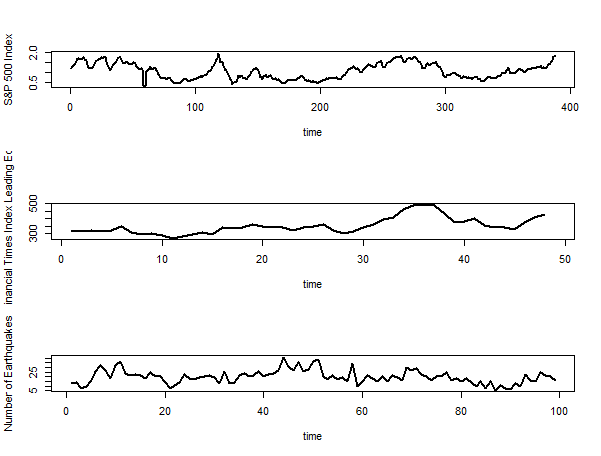
\includegraphics[width=3in]{realdata}
    \caption{Top: S\&P 500, Middle: Financial Times index leading equity, and Bottom: Number of Earthquakes per year}
    \label{realdata}
\end{figure}




\begin{table*}
    \centering
    \begin{tabular}{|c| c c c| c c c| c c c|}
        \hline
        Method & \multicolumn{3}{ c| }{Lag Orders (p,q)} & \multicolumn{3}{ c| }{Model Fit RMSE} & \multicolumn{3}{ c| }{Forecast RMSE} \\ 
        & QFT & SP500 & EQ & QFT & SP500 & EQ & QFT & SP500 & EQ\\\hline
        ABARMA & (4,2) & (1,0) & (1,0) & 18.374 & 0.099 & 6.128 & 65.921 & 0.407 & \textbf{6.915}\\\hline
        MLE & (10,9) & (10,10) & (10,10) & \textbf{9.770} & 0.093 & \textbf{4.818} & 81.732 & 0.409 & 7.204\\\hline
        CV & (1,0) & (0,0) & (7,10) & 23.457 & \textbf{0.403} & 4.910 & \textbf{51.335}& \textbf{0.403} &  7.142\\\hline
        AIC & (2,1) & (4,5) & (1,0) & 21.184 & 0.098 & 6.128 & 77.704 & 0.407 & \textbf{6.915}\\\hline
        AICc & (2,1) & (4,5) & (1,0) & 21.184 & 0.098 & 6.128 & 77.704 & 0.407 & \textbf{6.915}\\\hline
        BIC & (2,0) & (1,1) & (1,0) & 21.959 & 0.099 & 6.128 & 57.908 & 0.407 & \textbf{6.915}\\\hline
        \end{tabular}
    \caption{Results for real datasets of six different methods.}
    \label{tab:realres}
\end{table*}

\iffalse
We simulate $25$ mean zero series of $100$ observations from each of  model orders: $p, q = (2,1)$ and $(5,3),$ and simulated $20$ mean zero series of $100$ observations of model order $(8,6)$ which we label low, medium, and high order models respectively, using the {\tt arima.sim} function available by default in {\tt R}.  $100$ observations are used since the {\tt auto.arima} function approximated the maximum likelihood values when the number of observations exceeds $100$.  Examples of these series are shown in Figure \ref{sample}.

\begin{figure}
    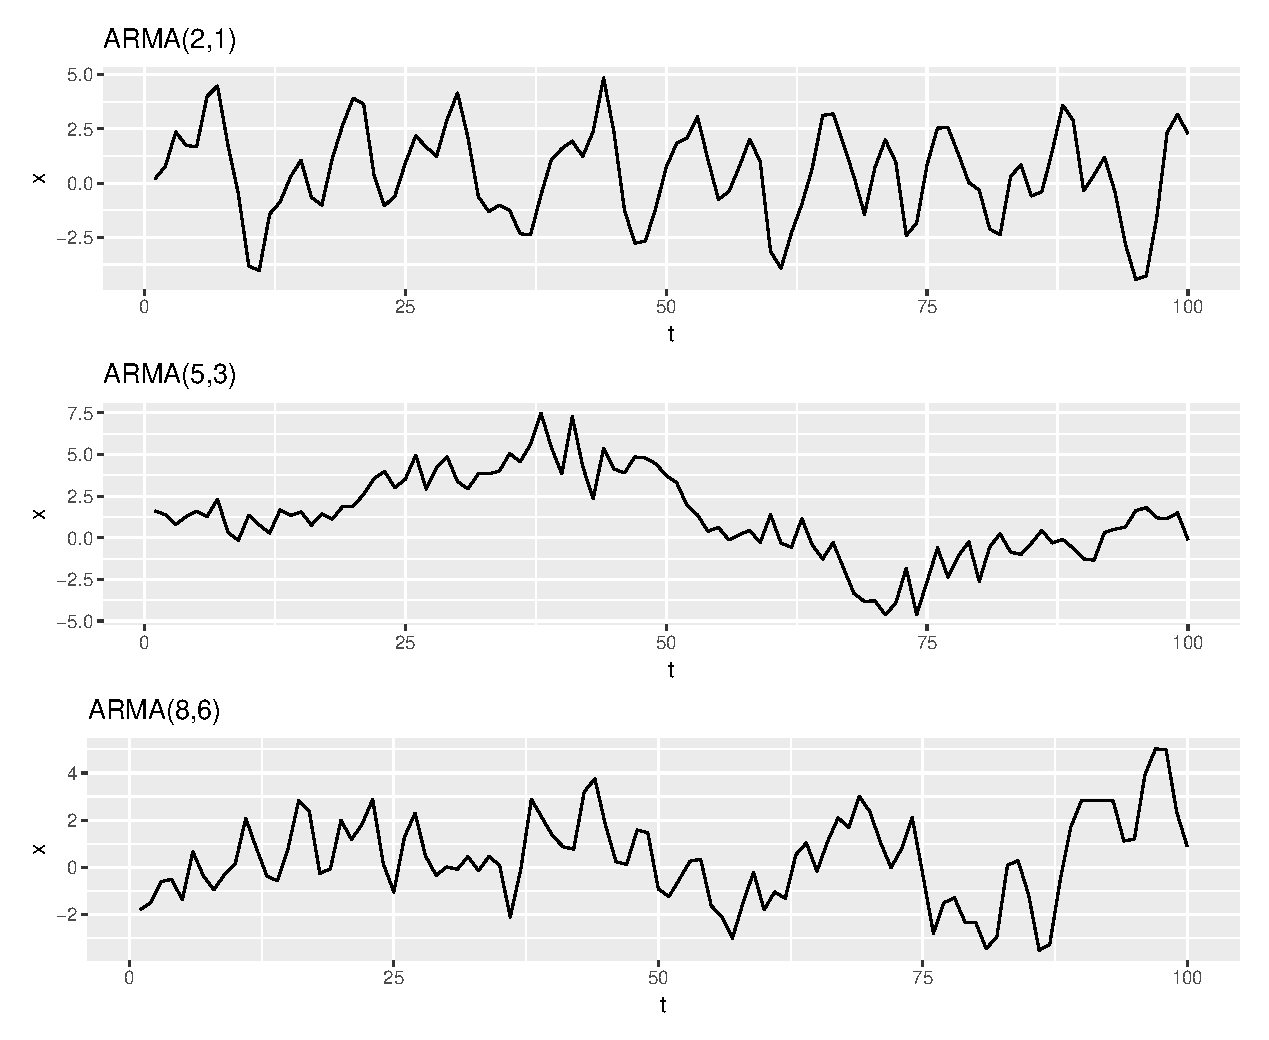
\includegraphics[width=3in]{armaLMH.eps}
    \caption{Top: ARMA$(2,1)$, Middle: ARMA$(5,3)$, Bottom: ARMA$(8,6)$}
    \label{sample}
\end{figure}


We contrast the ABARMA method with {\tt auto.arima} (a non-bayesian, but widely used approach) by comparing the recovered lag orders with the true model lag orders.  For low and medium orders, both models have maximum lag orders set to five, and for high order, both models have maximum lag orders set to ten.  We do not compare our model to that proposed in \cite{monahan1982} as it is based on numerical integration which is very slow.  The ABARMA method takes roughly $1$ minute with maximum $p$ and $q = 5$ on a standard desktop computer, while numerical integration of the integral in (3) takes slightly over $4$ minutes when setting convergence to $5000$ function evaluations. Furthermore, limiting the number of function calls reduces accuracy.  For ten simulated series with $p=2$ and $q=1$, numerical integration chose the correct AR order $40\%$ of the time and the correct MA order $30\%$ of the time, which is much worse than ABARMA and {\tt auto.arima} as shown in Figures \ref{ar21} and \ref{ma21} which achieve greater than $50\%$ accuracy for AR orders, and $56\%$ and $68\%$ for MA orders respectively. The {\tt auto.arima} function takes roughly $0.08$ seconds to run with maximum $p$ and $q=5$.

\begin{figure}
    \centering
    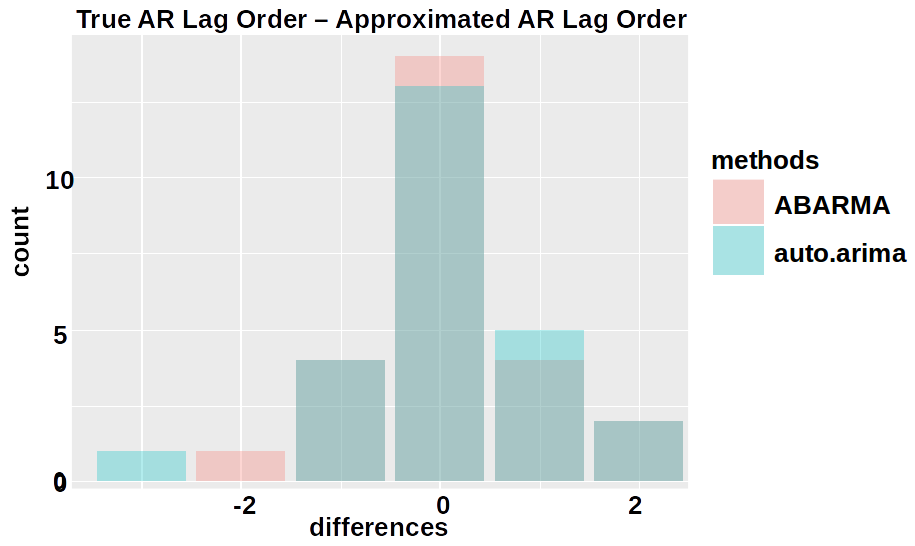
\includegraphics[width=3in]{ar21_new}
    \caption{AR order estimation error for low order model.}
    \label{ar21}
\end{figure}

\begin{figure}
    \centering
    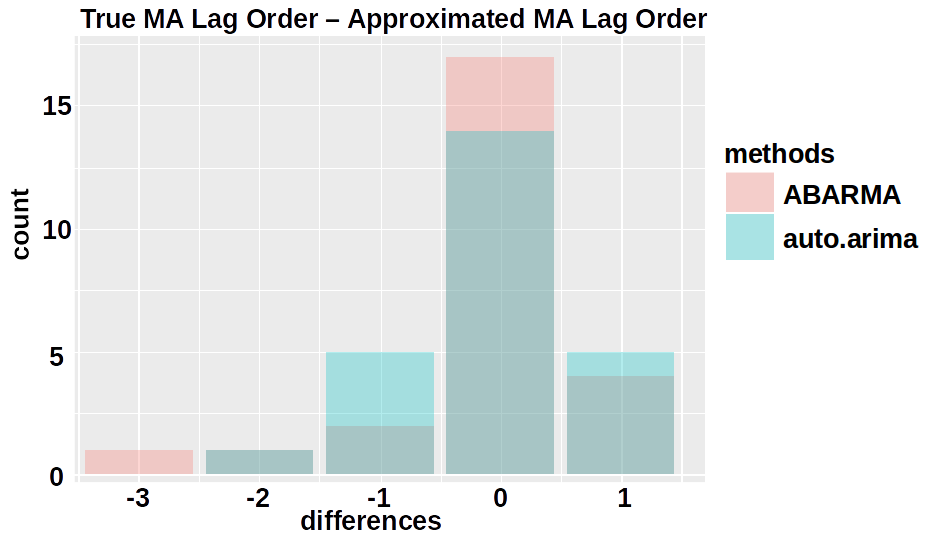
\includegraphics[width=3in]{ma21_new}
    \caption{MA order estimation error for low order model.}
    \label{ma21}
\end{figure}

In Figures \ref{ar21} and \ref{ma21}, we visualize the estimation error of the ABARMA model and {\tt auto.arima} function compared to the true model orders for small lag orders.  ABARMA (red) correctly estimates the true lag orders more often than {\tt auto.arima} (blue) and tends to favor larger model orders, especially for MA terms shown by the number of negative values in the plot.  

For medium order models the ABARMA model AR order is often much closer to the true model AR order than the {\tt auto.arima} function.  Again we see that the ABARMA method favors larger MA orders and finds the correct MA order more often than {\tt auto.arima}.

For high order models, the ABARMA model is significantly closer to the true model order than {\tt auto.arima}, though both models rarely give large AR orders.  For the AR order number, the {\tt auto.arima} function never selects an order number less than two away from the true model order, whereas the majority of model orders selected by ABARMA are within two.  Again, the ABARMA method favors larger MA order numbers, and is almost entirely within $\pm 3$ of the true order whereas a majority of {\tt auto.arima} terms are four or more away.

The top plots in Figures \ref{fig: medium} and \ref{fig: high} located in Appendix C visualize the results described above for medium and high order models..

\begin{figure}
    \centering
    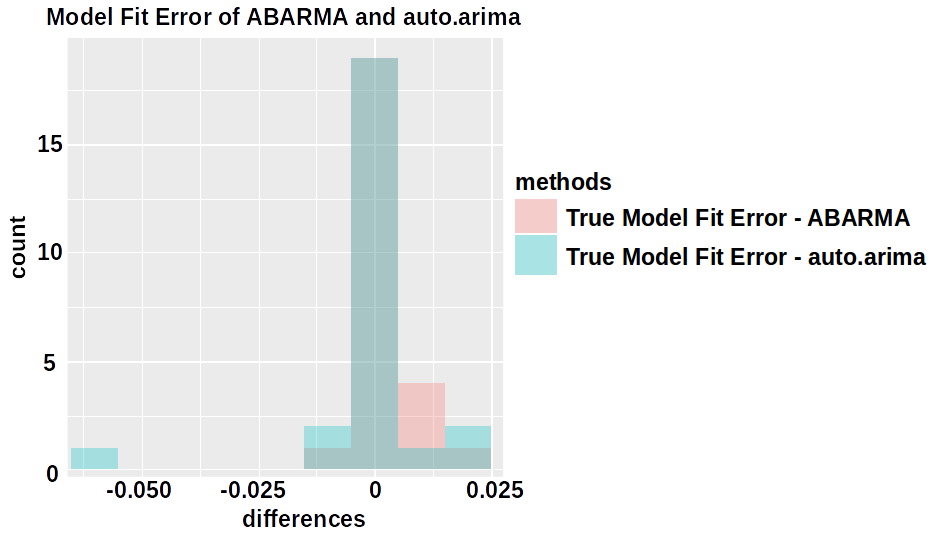
\includegraphics[width=3.25in]{mfrmse21_new.png}
    \caption{Difference in model fit error with true model for low order model.}
    \label{mfrmse21}
\end{figure}

\begin{figure}
    \centering
    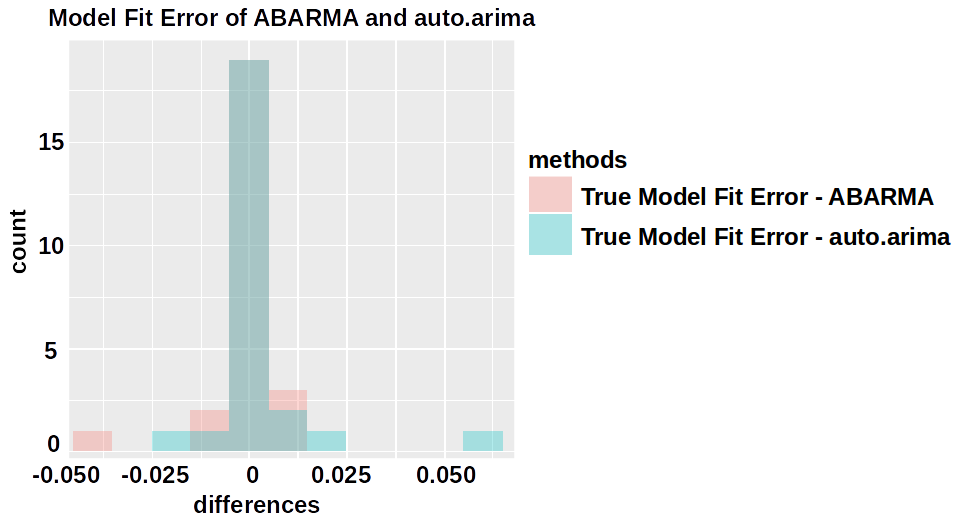
\includegraphics[width=3.25in]{fermse21_new.png}
    \caption{Difference in forecast error with true model for low order model.}
    \label{fermse21}
\end{figure}

Another quantitative evaluation of the relative strength of ABARMA is how well the model is able to fit and forecast series. We fit a model with lag orders determined by ABARMA, forecast the next $10$ observations of the series, and report the RMSE for each of the simulated series.  Figures \ref{mfrmse21} and \ref{fermse21} show the difference in RMSE for model fit and forecast error between the true model and ABARMA model (red), and between the true model and the {\tt auto.arima} model (blue) for low order models (i.e. error of true $p,q$ model - error of ABARMA or {\tt auto.arima} model in fitting and forecasting). For medium and high order models, the bottom plots in Figures \ref{fig: medium} and \ref{fig: high} in Appendix C visualize the difference.  In all models, ABARMA maintain both model fit and forecasted accuracy close to that of the true model, and similar to the model fit proposed by {\tt auto.arima}.  In most cases, both ABARMA and {\tt auto.arima} models have values close to zero, though in some cases values can be positive implying a fit which is better than the fit of the true model.  In some cases this might be due to the simulated model or withheld data being unusually noisy, or a poor forecast by all three methods.

The simulations suggest that ABARMA finds a good balance between estimating the correct lag orders and providing good fit to the data.
\fi
\iffalse
 One of the shortcomings of the {\tt auto.arima} function developed in \cite{hyndman2008} is that the algorithm favors models with smaller orders even when the data comes from a higher order ARMA model. For example, for a given process 
 
 \begin{align*}
     X_t &= 0.8897X_{t-1} -0.4858X_{t-2}  + 0.6X_{t-3} - 0.2X_{t-4}\\
     &+  0.1X_{t-5} - 0.2279\epsilon_{t-1}  +  0.2488\epsilon_{t-2} +  0.4\epsilon_{t-3} + \epsilon_t
\end{align*}
 
 the {\tt auto.arima} function selects an ARMA$(3,0)$ model.  
 
 We can readily generate small, medium, and high order ARMA process data via available {\tt R} functions such as {\tt arima.sim}.  This function is built into the package {\tt forecast} which also has the {\tt auto.arima} function.  We will extensively test on simulated data the results of our algorithm in better selecting medium and higher order processes.
 \fi
  

\iffalse
\begin{enumerate}
    \item Quarterly Financial Times index leading equity, 1960-1971 49
    \item Quarterly S\&P 500 index, 1900-1996 100
    \item Number of earthquakes per year magnitude 7.0 or greater, 1900-1998 389
\end{enumerate}
\fi

\iffalse
For each dataset, we fit the model as determined by ABARMA. and check the appropriateness of the ARMA model fit through residual analysis. A series of four plots for the residuals are used to verify that the residuals are independently and identically normally distributed, per our model assumption.

We compare model fit and forecast accuracy with {\tt auto.arima}.  The forecasted values consist of the most recent $5\%$ of the data which is omitted from training the model.
\fi
\iffalse
We can empirically analyze our algorithm on a number of time series datasets and compare to existing strategies.  Some popular datasets include those available at the Time Series Data Library created by Rob Hyndman \url{https://datamarket.com/data/list/?q=provider:tsdl} and the popular M3 forecasting competition dataset available at \url{https://forecasters.org/resources/time-series-data/m3-competition/}. 
\fi
\iffalse
\subsection{Dataset 1: Financial Times index leading equity}

ABARMA finds an ARMA$(2,1)$ model and {\tt auto.arima} finds an ARMA$(1,3)$ model.  The resulting model fit RMSEs for  {\tt auto.arima} and ABARMA respectively are  $20.44070$ and  $20.47979$, and the forecast errors are $33.79902$ and  $30.64232$.  In this example the model found by ABARMA performs better at forecasting than that found by {\tt auto.arima}.

\begin{figure}[h]
    \centering
    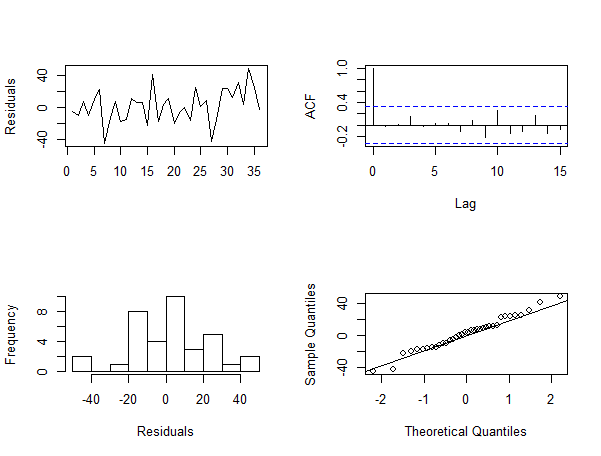
\includegraphics[width=3.5in]{diagnostics_fin.png}
    \caption{Residual analysis for ABARMA model fit for Financial Times index. Top left: plot of residuals. Top right: autocorrelations of residuals. Bottom left: histogram of residuals. Bottom right: Q-Q plot of residuals.}
    \label{fig: fin}
\end{figure}

Figure \ref{fig: fin} shows that the residuals appear independently normally distributed, and hence does not violate our model assumption.

\subsection{Dataset 2: S\&P 500 index}

%1.00000000 1.00000000 1.00000000 1.00000000 0.09418076 0.09418092 0.38579952 

Both ABARMA and {\tt auto.arima} find an ARMA$(1,1)$ model.  The resulting model fit RMSEs for  {\tt auto.arima} and ABARMA respectively are  $0.09418076$ and  $0.09418092$, and the forecast errors are $0.38579952$ and $0.38579649$.  We note that although both methods are identical the slight difference in RMSE is likely due to the {\tt auto.arima} implementation being slightly different from the standard {\tt arima} function in {\tt R}.


\begin{figure}[h]
    \centering
    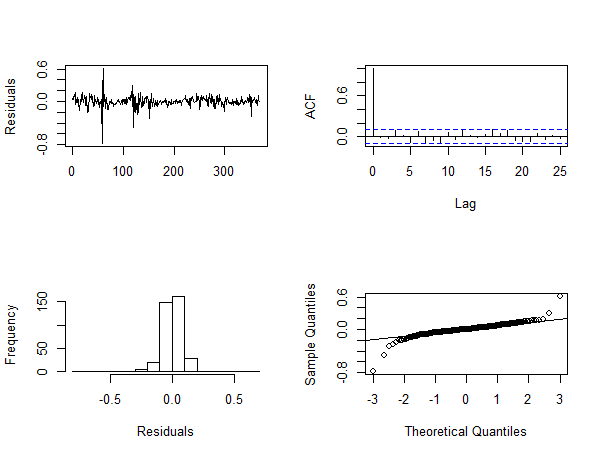
\includegraphics[width=3.5in]{daignostics_sp500.png}
    \caption{Residual analysis for ABARMA model fit for S\&P 500 index. Top left: plot of residuals. Top right: autocorrelations of residuals. Bottom left: histogram of residuals. Bottom right: Q-Q plot of residuals.}
    \label{fig: sp500}
\end{figure}

Figure \ref{fig: sp500} shows that the residuals appear independently normally distributed, and hence does not violate our model assumption.

\subsection{Dataset 3: Number of earthquakes per year}

Both ABARMA and {\tt auto.arima} find an ARMA$(1,0)$ model.  The resulting model fit RMSEs for  {\tt auto.arima} and ABARMA respectively are  both $6.256162$, and the forecast errors are $4.718671$.  Both models fit identically.

\begin{figure}[h]
    \centering
    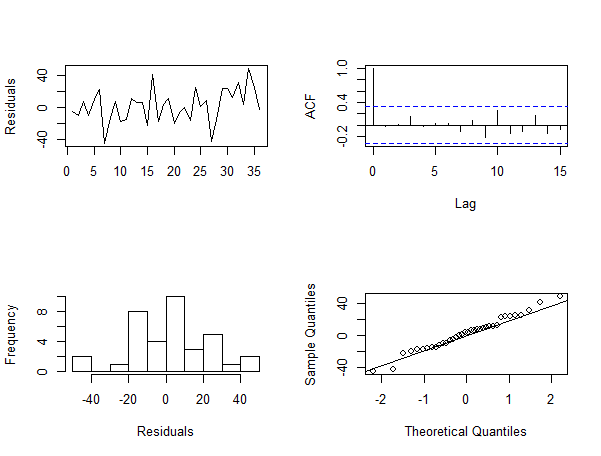
\includegraphics[width=3.5in]{diagnostics_eq.png}
    \caption{Residual analysis for ABARMA model fit for number of earthquakes per year. Top left: plot of residuals. Top right: autocorrelations of residuals. Bottom left: histogram of residuals. Bottom right: Q-Q plot of residuals.}
    \label{fig: earth}
\end{figure}

Figure \ref{fig: earth} shows that the residuals appear independently normally distributed, and hence does not violate our model assumption.
\fi
\iffalse
\subsection{Alternative Approximation}
We simulate sets of points from within the triangular pyramid described in section 6.  In 1000 simulated trials we simulated hundreds of points from within the region (since the region is hard to simulate exactly even for $C_3$ some points are thrown out).   Of those within the triangular pyramid $\approx 84.3\%$ were in $C_3$.  These results show that the approximated region is a good first step approximation, however the actual region is more complicated, and a better approximation is needed.
\fi

%\section{Future Work}



\iffalse
We summarize remaining work to be done for the project:
\begin{itemize}
    \item Explore better approximation to $C_p \times C_q$ and generalize the current approximation to $p>3$.
\end{itemize}

In practice the Hessian matrix must be computed recursively as the derivatives of $\tilde{\mu}_t$ rely on previous derivatives of $\tilde{\mu}$.  


using different function for $\tilde{r}$

better approximation/generalized approximation for space
\fi 

\section{Conclusion}
\label{sec: conclusion}

In this paper, we introduced ABARMA, a Bayesian approach to determine the lag orders $p$ and $q$ of ARMA models. Laplace approximation is used to reduce the computational burden of numerical integration present in previous Bayesian treatments of the problem.

We extensively compared implementations of ABARMA with {\tt auto.arima} on simulated and real-world. Results show that ABARMA determines the lag orders more accurately than other methods, and places high probability only around the true lag orders, while all other methods place a more uniform distribution over all $p$ and $q$.  The method is also fairly robust to noise and initialization and increases in accuracy with the length of the time series while runtime scales linearly.  Fit and forecast errors of models determined by ABARMA are at least comparable to those of other methods.

ABARMA performs an exhaustive search for the optimal lag orders. The algorithm can be sped up by considering more efficient strategies such as Bayesian optimizaation as in \cite{snoek2012},  \cite{bergstra2011}, and \cite{snoek2015} and as already shown by the step-wise procedure in Section \ref{sec:speedups}.  While Bayesian optimization does scales with dimension, it was proved in \cite{kandasamy2015} that the regret is only linear in the dimension, and the dimension $D$ is still relatively small ($D \leq 21$). Another possibility for ABARMA is to consider more general approximation techniques such as  variational inference \cite{blei2016variational}.  Variational inference has the advantage of allowing more flexible approximating distributions and does not place as heavy an emphasis on the mode of the distribution as does Laplace.


\iffalse

\section{Future Work}
\label{sec: fw}

There are several directions of possible future work.  First, while in most cases our method is overall closer to the true lag orders, we want to examine more closely the behavior of ABARMA in selecting MA coefficients above the true orders as seen in Figures \ref{fig: medium} and \ref{fig: high}.  It is especially interesting to us that no method overshoots the AR coefficient for medium and high true orders, however ABARMA overshoots the MA true order significantly in the true medium order case as Bayesian models tend to be parsimonius and favor simplicity.

Second, our current optimization procedure performs an exhaustive search for the optimal lag orders.  The algorithm takes roughly 1-3 seconds for approximating the evidence for a given (medium) value of $p$ and $q$.  Thus exhaustively computing for every $p$ and $q$ becomes a major bottleneck when we consider $120$ configurations (maximum $p$ and $q=10$).  We can speed up this major bottleneck of the algorithm by considering more efficient strategies such as Bayesian optimizaation \cite{snoek2012} or step-wise as in \cite{hyndman2008}.  While Bayesian optimization does scales with dimension, it was proved in \cite{kandasamy2015} that the regret is only linear in the dimension, and the dimension $D$ is still relatively small ($D \leq 21$). 


Finally, we note that our approximation is based on Laplace method.  Although the Laplace approximation appeared to fit $f(\theta^*)$ well according to Figure \ref{fig:laplace} we would like to consider more general approximation techniques such as  variational inference \cite{blei2016variational}.
\fi

\begin{acks}
We thank the anonymous reviewers of ORIE 6741 for their helpful feedback and discussions.  
\end{acks}


\bibliographystyle{ACM-Reference-Format}
\bibliography{ABARMA.bib} 

\end{document}
